\begin{figure}

\caption{The Three-Dimensional Model Exported 
from 3DimViewer to MeshLab}
\label{fig:rad3}

\begin{tikzpicture}

%\nodeincludegraphicsTR{2.7cm}{2cm}{pics/RAD-2.png}

\node[inner sep=0pt] (r3) at (0,0)
    {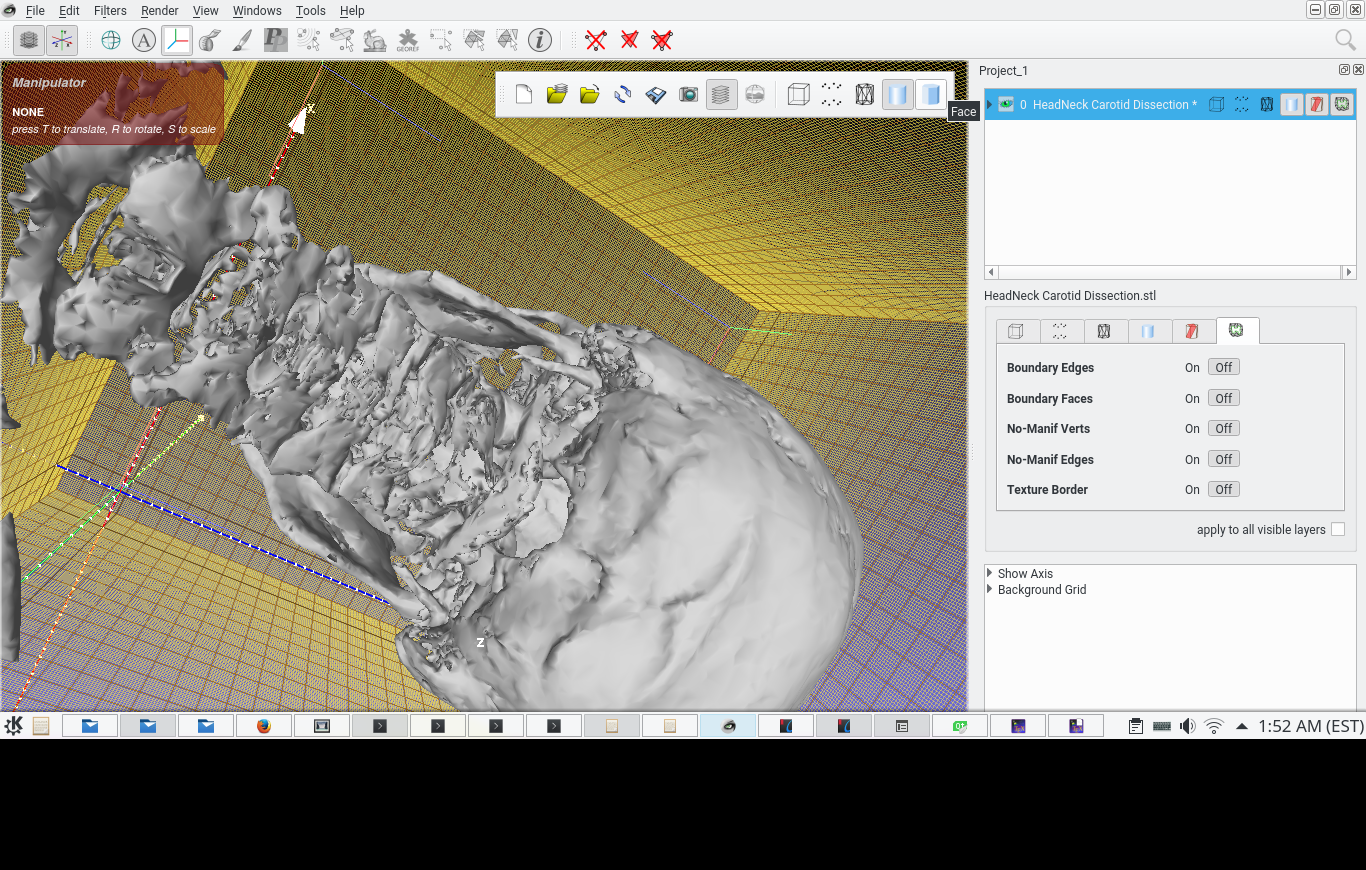
\includegraphics[width=7.5in,%width=0.7\pagewidth, 
    	trim={0mm 40mm 0mm 0mm},clip]
    	{pics/Rad-3.png}};

% \node [anchor=west,fill=brown!20!white,inner sep=7, text width=14cm]
%  (longnote) at (5.5,7) {%  %{\color{rb!85!red}{
%  {\cframedbox{\large \textbf{EC3}}}};

 \node [anchor=west,bottom color=brown!80!purple,
 top color=white, %top color=blue!40!cyan, 
 shading angle=310, 
 inner sep=6, text width=12.6cm]
  (longnote) at (-8,-4) {%\vspace{-8pt}%  %{\color{rb!85!red}{
  {\textbf{MeshLab's 
enhanced ability to receive data from other application 
augments its value as a general-purpose 3D graphics viewer.}}};

\end{tikzpicture}


\end{figure}

